\documentclass[11pt]{beamer}


\usepackage[utf8]{inputenc}
\usepackage[czech]{babel}
\usepackage{times}
\usepackage{graphics}
\usepackage[ruled, czech, linesnumbered, noline, longend]{algorithm2e}
\setbeamertemplate{footline}[frame number]
\setbeamertemplate{headline}{}
\title{Typografie a~publikování\,--\,5.~projekt}
\subtitle{Řadicí algoritmy}
\author{Assatulla Dias \\\smallskip \tiny{xassat00@stud.fit.vutbr.cz}}
\date{\today}


\begin{document}
\maketitle
\setbeamercovered{transparent}
\begin{frame}{Přehled}
 \begin{enumerate}[(I)]
     \item \uncover{Úvod a Motivace}
     \pause
     \item \uncover{Bublinkové řazení a příklad}
     \pause
     \item \uncover{Složitost algoritmu}
 \end{enumerate}
\end{frame}

\begin{frame}{Úvod}
    \begin{itemize}
        \item Řadicí algoritmus\,--\,je algoritmus pro řazení prvků v poli. V případě, že prvek v poli má více polí, pole, které slouží jako kritérium pořadí, se nazývá klíč řazení. 
        \item V praxi číslo často funguje jako klíč a zbývající pole ukládají všechna data, která neovlivňují činnost algoritmu.
    \end{itemize}
\end{frame}

\begin{frame}{Motivace}
    \begin{itemize}
        \item Představte si, že máte knihu, která obsahuje seznam jmen všech postav ve vesmíru Disney. Ale všechna jména jsou v této knize pomíchaná. Což znamená, že postava Jafara by mohla být v první řadě této knihy nebo uprostřed nebo na konci. A chcete najít postavu Maleficent. Budete muset zkontrolovat každý řádek v této knize, abyste našli to, co chcete. 
        \item Nepohodlné a ztráta času, že? Bylo by mnohem jednodušší, kdyby byl seznam v knize řazen abecedně a vy byste přešli přímo na seznam začínající písmenem M.
    \end{itemize}
\end{frame}

\begin{frame}{Tak proč potřebujeme řadicí algoritmy?}
    \begin{itemize}
        \item Efektivní řazení je důležité pro optimalizaci účinnosti jiných algoritmů (jako jsou search a merge algoritmy), které vyžadují, aby vstupní data byla v setříděných seznamech.
        \item Produkce čitelnějšího výstupu.
        \item Je snazší a rychlejší najít položky v seřazeném seznamu než v neseřazeném.
    \end{itemize}
    \bigskip
    Pro své prezentace jsem zvolil \uv{\,bubble sort\,}.
\end{frame}

\begin{frame}{Bublinkové řazení (Buble Sort)}
    \begin{itemize}
        \item Bublinové řazení provede několik průchodů seznamem. Porovnává sousední prvky a zaměňuje ty prvky, které jsou ve špatném pořadí. 
        \item Každý průchod seznamem umístí další největší hodnotu na správné místo. V podstatě každý prvek \uv{\,bublá\,} na své místo.
    \end{itemize}
    \begin{figure}
        \centering
        \scalebox{0.4}{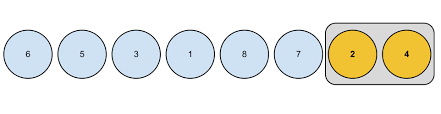
\includegraphics{bubleImg/buble1.png}}
        \label{fig:Buble_Sort}
    \end{figure}
\end{frame}

\begin{frame}{Příklad}
    \begin{itemize}
        \item Představte si, že máte seznam lidí, které chcete seřadit podle věku, od nejmladších po nejstarší.
        \item Seznam věků je: 54, 26, 93, 17, 77, 31, 44, 55, 20.
    \end{itemize}
    \begin{figure}
        \centering
        \scalebox{0.7}{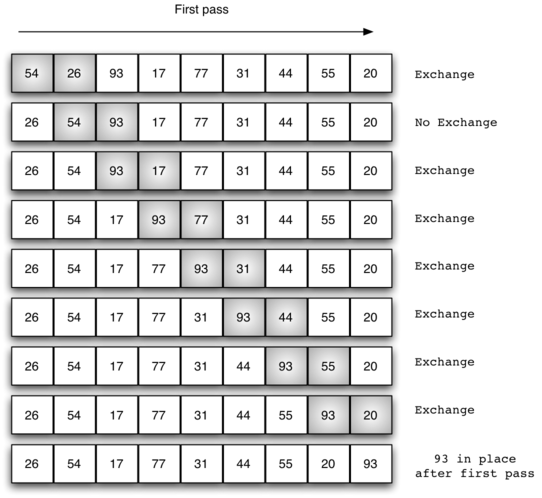
\includegraphics{bubleImg/bubblepass.png}}
        \caption{Buble sort: 1. průchod}
        \label{fig:Buble_Sort_Example}
    \end{figure}
\end{frame}
\begin{frame}{Příklad pokr.}
    
    \begin{itemize}
        \item Obrázek \ref{fig:Buble_Sort_Example} ukazuje první průchod bublinového typu. Stínované prvky budou porovnány, aby se zjistilo, zda jsou ve správném pořadí. Pokud je v seznamu \(n\) prvků, pak bude potřeba pár \(n-1\) porovnat v prvním průchodu. Je důležité poznamenat, že protože největší hodnota je součástí dvojice, bude se pohybovat po seznamu, dokud nebude průchod dokončen.
    \end{itemize}
    \begin{figure}
        \centering
        \scalebox{0.145}{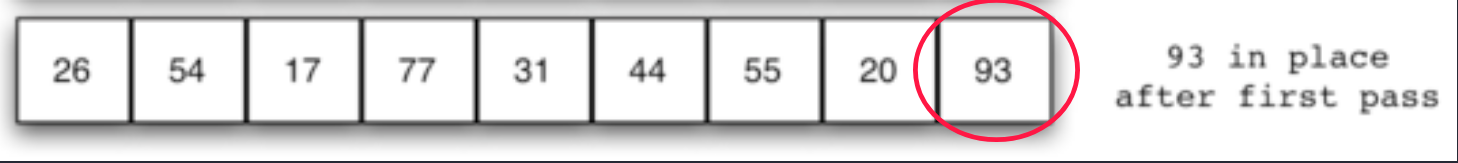
\includegraphics{bubleImg/bublepass_2.png}}
        \caption{Výsledek po prvním průchodu}
        \label{fig:Buble_Sort_Example_2}
    \end{figure}
    \begin{itemize}
        \item Na začátku druhého průchodu je na svém místě nejvyšší hodnota. To zbývá seřadit \(n-1\) čísla nebo \(n-2\) páry. Protože každý průchod umístí další největší hodnotu na správné místo, celkový počet průchodů je \(n-1\). Po dokončení \(n-1\) průchodu bude nejmenší prvek ve správné poloze bez dalších výpočtů.
    \end{itemize}
   
\end{frame}

\begin{frame}{Pseudokód algoritmu}
    \begin{algorithm}[H]
        \label{algorithm:Buble_Sort}
        \caption{\textsc{Buble Sort}}
        \KwData{Input Array $A[]$}
        \KwResult{Sorted $A[]$}
        $int\,i, j, k;$ \\
        $N = lenght(A);$ \\
        \For{$j = 1\;to\;N$} {
            \For{$i = 0\;to\;N-1$}{
                \If{$A[i] > A[i+1]$}
                {
                    $temp = A[i];$ \\
                    $A[i] = A[i+1];$ \\
                    $A[i+1] = temp;$ 
                }
            }
        }
    \end{algorithm}
\end{frame} 

\begin{frame}{Složitost algoritmu}
    \begin{itemize}
        \item Tento algoritmus je považován za výukový a ve své čisté podobě se v praxi téměř nepoužívá. Jde o to, že průměrný počet kontrol a permutací v poli je počet prvků na druhou. Například pole 10 prvků by vyžadovalo 100 kontrol, zatímco pole 100 prvků by vyžadovalo stokrát tolik, 10 000 kontrol.

        \item Ukazuje se, že pokud máme v poli 10 tisíc prvků (a to není příliš velké pole, pokud jde o skutečné IT úkoly), pak jeho třídění bude vyžadovat 100 milionů kontrol - bude to nějakou dobu trvat. Ale co když potřebujete řadit několikrát za sekundu?

        \item V programování se účinnost algoritmu v závislosti na počtu prvků n označuje takto: $O(n)$. V našem případě je výkon bublinového řazení $O(n^2)$. Ve srovnání s jinými algoritmy se jedná o velmi velký indikátor (čím větší, tím více času zabere řazení).
    \end{itemize}
\end{frame}

\end{document}